\chapter{Mischer}
\label{ch:concept}
\section{Allgemeines}
Der Audio Mixer verknüpft verschiedene, von den anderen Bauteilen des modularen Synthesizers erzeugte Eingangssignale (Klangquellen) miteinander. Das heißt er mischt, kombiniert und gleicht verschiedene Klänge und Audiosignale aus, wodurch neue Signalformen
und Klänge generiert werden können. Die entstehenden kombinierten Signale werden an den Filter weitergeleitet.


\section{Schaltplan}
Dieser Abschnitt beschreibt den Schaltplan des Mischers in Abbildung \ref{fig:schaltplan_mixer}. 
Dazu werden die einzelnen Teilbereiche des Schaltplans vorgestellt.

IN1-IN3 sind die Audioeingangsbuchsen, INV OUT-CLIP OUT sind die Audio-Ausgangsbuchsen.

Der Teilbereich 1 des Schaltplans ermöglicht die Anpassung der Lautstärke der Signale in jedem Bereich zwischen 0\% und 100\%. 
Ein zentrales Bauteil ist der Vierfach-Operationsverstärker TL074P. Die drei verbauten Potentiometer regeln die Levels der Eingangssignale.

Der zweite Teilbereich lässt eine Modulation des Ausgangssignals (hinsichtlich Verzerrung und Wärme des Klangs) zu. Der Strom fließt durch die Diode nur in eine Richtung. Der 100k-Widerstand wird benötigt, um die Gefahr eines Kurzschlusses zu beheben. Denn ohne diesen Widerstand würde der Strom exponentiell steigen, da sich die Diode unbegrenzt öffnet, wenn die Spannung ansteigt. Die Spannung über der Diode bleibt konstant, wenn der Operationsverstärker einen bestimmten Threshold übersteigt. Dieser Effekt nennt sich Soft Clipping. Die zweite verbaute Diode erfüllt einen entsprechenden Zweck für negative Spannung. 
In Teilbereich 3 ist XP1 ein Standard-Eurorack-Stromanschluss. Es handelt sich um eine 2x5-Stiftleiste mit einem Schlüssel, die eine versehentliche Stromversorgung mit umgekehrter Polarität verhindern soll, denn ein falscher Anschluss der Stromversorgung würde zu dauerhaften Schäden am Modul führen. D3 und D4 sind Schottky-Dioden, die die Stromversorgung mit umgekehrter Polarität doppelt sichern.
Auf den + und -12-V-Schienen wurden zwei 10-Ohm-Widerstände (R15 und R16) mit Entkopplung verwendet und Kondensatoren C1 - C4. In Kombination mit R15 und R16 kompensiert C1 und C2 Niederfrequenzschwankungen, während C3 und C4 Funkfrequenzen, Hochfrequenzspitzen von Schaltnetzteilen und schnelle, von anderen Modulen erstellte Spitzen herausfiltern.
Die Kondensatoren C5 - C8 sind zusätzliche Entkopplungskondensatoren.

\begin{figure}[h]
	\centering
	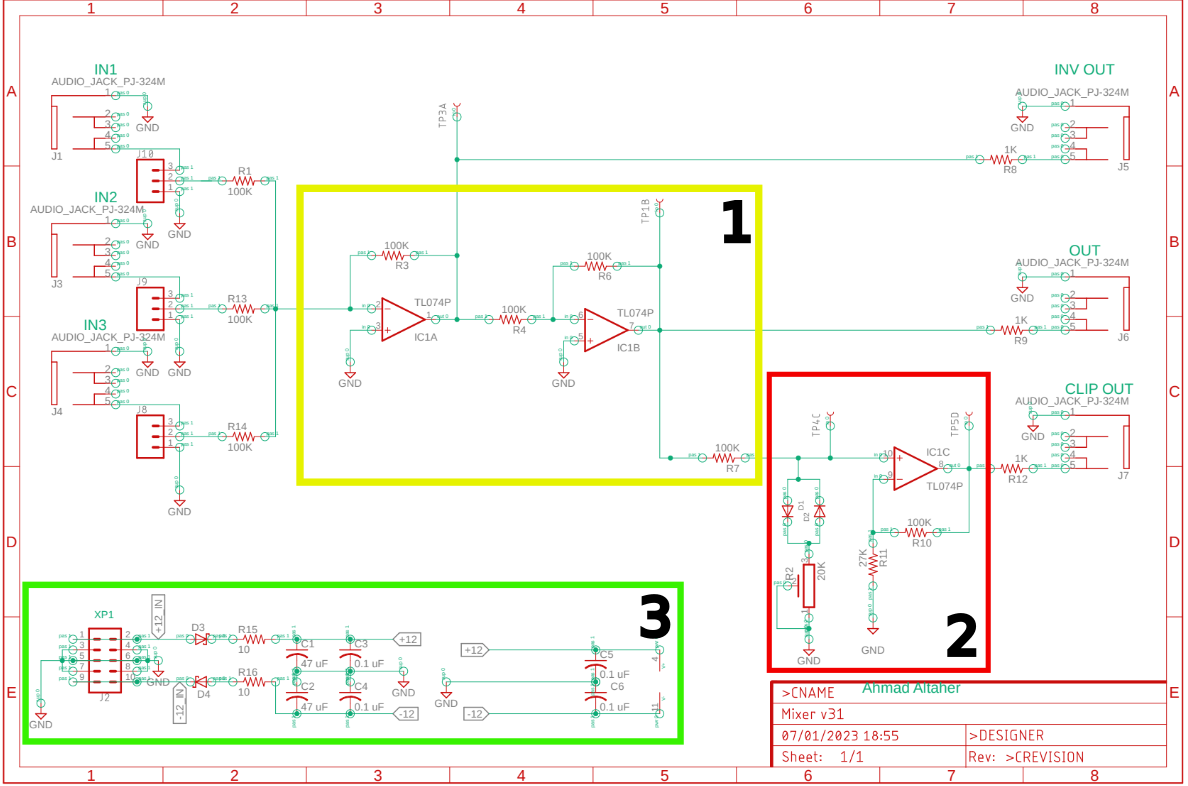
\includegraphics[angle=270, width=1\textwidth]{figures/SchaltplanMixer_new.png}
	\caption{Ausschnitt des Mischer-Schaltplanes aus Fusion360 \cite{mixer_manual}}
	\label{fig:schaltplan_mixer}
\end{figure}
\FloatBarrier

\section{Platine}
\begin{figure}[h]
	\centering
	\setlength{\fboxsep}{1pt} %Abstand der Linien zur Abbildung
	\setlength{\fboxrule}{1pt} %Dicke der Linie
	\fbox{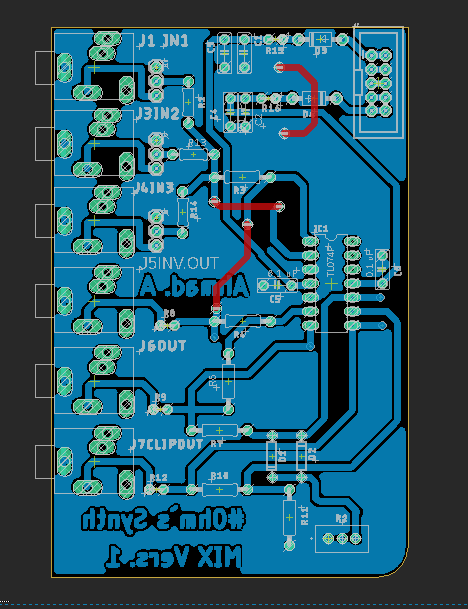
\includegraphics[width=0.7\textwidth]{figures/mixer_platine.png}}
	\caption{Ausschnitt des Mischer-Platinen-Layouts aus Fusion360 (Unterseite)}
	\label{fig:platine_mixer}
\end{figure}
\FloatBarrier